\documentclass[12pt]{article}

\usepackage{float}

\usepackage{standalone}

%\usepackage[utf8x]{inputenc}

%%% PAGE DIMENSIONS
\usepackage{geometry}
\geometry{a4paper}
\geometry{margin=2.54cm} % for example, change the margins to 2 inches all round

\usepackage{graphicx} % support the \includegraphics command and options

\usepackage[parfill]{parskip} % Activate to begin paragraphs with an empty line rather than an indent

%%% PACKAGES
\usepackage{booktabs} % for much better looking tables
\usepackage{array} % for better arrays (e.g., matrices) in maths
\usepackage{paralist} % very flexible & customisable lists (e.g., enumerate/itemise, etc.)
\usepackage{verbatim} % adds environment for commenting out blocks of text & for better verbatim
\usepackage{subfig} % make it possible to include more than one captioned figure/table in a single float
% These packages are all incorporated in the memoir class to one degree or another...

\usepackage{multicol}
\usepackage{multirow}
\usepackage{xcolor}
\usepackage{amsmath}

\usepackage[T1]{fontenc}
\usepackage{lmodern}

% Sans-serif font
\renewcommand{\familydefault}{\sfdefault}

\usepackage{makecell}

\renewcommand{\arraystretch}{1.1}

%%% HEADERS & FOOTERS
\usepackage{fancyhdr} % This should be set AFTER setting up the page geometry
\pagestyle{fancy} % options: empty , plain , fancy
\fancyhead[L]{\leftmark}
\fancyhead[C]{}
\fancyhead[R]{\rightmark}
\fancyfoot[L]{}
\fancyfoot[C]{}
\fancyfoot[R]{\thepage}
\renewcommand{\headrulewidth}{0pt}
\renewcommand{\footrulewidth}{0pt}
\setlength{\headheight}{52pt}

\fancypagestyle{plain}{
	\fancyhf{} % clear all header and footer fields
	\fancyfoot[R]{\thepage} % except the center
	\renewcommand{\headrulewidth}{0pt}
	\renewcommand{\footrulewidth}{0pt}
}

%%% BIBLIOGRAPHY
\usepackage[numbers]{natbib}
\bibliographystyle{vancouver}

%%% SECTION TITLE APPEARANCE
\usepackage{sectsty}
\allsectionsfont{\sffamily\mdseries\upshape}

%%% ToC (table of contents) APPEARANCE
%\usepackage[nottoc,notlof,notlot]{tocbibind} % Put the bibliography in the ToC
%\usepackage[titles,subfigure]{tocloft} % Alter the style of the Table of Contents
%\renewcommand{\cftsecfont}{\rmfamily\mdseries\upshape}
%\renewcommand{\cftsecpagefont}{\rmfamily\mdseries\upshape} % No bold!

\usepackage[bookmarks,bookmarksnumbered,bookmarksopen,hidelinks]{hyperref}

\usepackage{bookmark}


%%% TITLE
\title{Statistical modelling of antibody data}
\author{Arseniy Khvorov, David J. Price, Annette Fox, Sheena G. Sullivan}
\begin{document}

%%% Title
\maketitle

%%% Main Contents

%==============================================================================
\section{Introduction}

In the study of infectious diseases it is useful to have some measure of whether a person is infected, immune or susceptible to infection. This may be important, for example, to understand disease prevalence, population-level susceptibility or for evaluation of vaccines.  However, direct measurement of immunity is often not possible and instead some \textit{correlate} of protection is used. For viral infectious diseases, an oft-used correlate is the serum antibody titre, which provides a measure of the amount of antibody that recognizes a particular epitope. 

Antibody titres have several limitations. Titres are the inverse of the greatest dilution of antibody that inhibits virus in serial dilutions, with higher values indicating greater inhibition. There is no true zero value, nor is there a true measure of the maximum value; titres can only be as low as the minimum starting concentration and as high as the maximum dilution.  Furthermore, within dilution intervals, the true concentration that inhibits virus is unknown; only the upper and lower bound of each dilution is known, i.e. titres are interval-censored. In addition, antibody titres are merely a surrogate measure and their sensitivity and specificity may be imperfect, such that reduced titres may not always correspond to increased susceptibility. 

For influenza, the haemagglutination inhibition (HI) antibody titre is an established correlate of protection. Indeed, the annual reformulation of influenza vaccines is partially dependent on demonstration that circulating viruses are no longer inhibited by vaccine-induced antibodies indicated by HI titres below a certain threshold \citep{Barr;2014}. And annual re-licensing of updated formulations is dependent on demonstrating that a vaccine induces HI titres above this same threshold \citep{Wood;2003}.  The HI threshold commonly used is a titre of 1:40, thought correspond to a 50\% reduction in risk. This figure is derived from cohort studies among vaccinated or infected individuals who have been followed for infection, and among whom the median titre associated with protection (no detected infection) is calculated \citep{Hobson;1972, Ng;2013}. 

%This threshold is also used to interpret susceptibility to infection among unvaccinated individuals for modelling studies and public health interventions. For example during the 2009 pandemic, age-specific susceptibility, established by sero-epidemiology studies \citep{Hardelid;2011}, helped direct targeted vaccination programmes %[need ref]. 

Several methods have been proposed for the analysis of antibody titre data and the calculation of protective thresholds. Each has its own set of assumptions that makes it more or less appropriate for the data being analysed. Here we will consider 3 models that are used in the literature: a Cox proportional hazards regression; a logistic regression; and a scaled logit model. Using simulations and data from two published studies, we discuss these models' assumptions, limitations and situations in which they may not be appropriate.


%==============================================================================
\section{Study designs and motivating examples}

Establishment of the threshold at 40 is based on human challenge studies from the 1960s in which volunteers were either randomised to received vaccine or not, or were challenged with virus \citep{Hobson;1972}. Blood samples were collected pre-challenge. For vaccinated individuals, challenge occurred at least 14 days after vaccination. Nasal swabs taken 48-hours after challenge were used to determine infection by virus culture, and for unvaccinated volunteers challenged with live virus, infection was additionally indicated by pre-to-post-challenge sero-conversion (4-fold rise in titre). In both cases, the protective titre was estimated from the pre-challenge geometric mean titre for uninfected participants. 

While challenge studies permit close observation of participant responses to infection under highly controlled conditions, the infectious dose administered may be unnaturally high. Several observational studies have been established to understand influenza transmission in more realistic conditions. In these studies, participants are determined to be at risk of infection because one or more of their close contacts (i.e. household members) has been identified as influenza-infected or because influenza has been known to be circulating.  Infection may be determined by laboratory testing of respiratory samples, or, if unvaccinated, by sero-conversion. In this paper, we will illustrate our findings using two established household studies. 


%------------------------------------------------------------------------------
\subsection{The Kiddivax study}

The Kiddivax study was a randomised controlled trial undertaken in Hong Kong in 2009-2010 in which 796 children aged 6-17 years were randomised to receive inactivated vaccine. We direct the reader to \citep{Cowling;2013} for full detail of the study but provide a brief outline here.

Blood samples were taken pre- and 1-month post-vaccination to estimate their vaccine-induced antibody titres.  The children and their household contacts were followed for approximately 7 months for influenza-like illness. Symptoms reported by any household member prompted swabbing and influenza testing by PCR for all household members \citep{Cowling;2013}. The protective titre was estimated using a Cox proportional hazards model where the outcome was time to infection or the end of the study \cite{Ng;2013}.


%------------------------------------------------------------------------------
\subsection{The Ha Nam household study}

%Antibody titres induced by vaccination may reach neither the concentration nor the breadth of antibodies induced by natural infection. Thus, the median titre indicative of protection post-vaccination may differ from the protective titre induced by prior infection among unvaccinated individuals. 
The Ha Nam study has followed 270 households in Ha Nam Vietnam since 2007. We direct the reader to \cite{Horby;2012} for full description of the study but provide a brief outline here.

Sera are collected (bi)annually, at intervals spanning RT-PCR-confirmed transmission periods, determined by surveillance data. Households are followed weekly for influenza-like illness and all household members swabbed when any member shows symptoms. Unlike the Kiddivax study, where the time at risk can be measured, in the Ha Nam study and other household studies of natural infection, the true time at risk is unknown. These differences are depicted in Figure \ref{Studies}.


%==============================================================================
\section{Models}

We will discuss all 3 models in the context of a binary outcome $Y$ representing the infection status where 0 --- not infected, 1 --- infected, and a continuous covariate $X$ representing the log-titre measurement. The fitting of all models will be done using the standard maximum likelihood framework. 

All observations with missing values will be removed. All censored titre observation will be handled as follows: below-detectable values will be set to half of the lowest detectable level (lowest detectable level is 10, so the below-detectable values are "imputed" as 5), above-detectable values will be set to the highest dilution used, the other values will be set to the geometric mean of the corresponding interval, e.g. a value of 20 would be shifted to the geometric mean of 20 and 40.


%------------------------------------------------------------------------------
\subsection{Cox proportional hazards}

The Cox PH is a common approach to analysing time-to-event data \cite{George;2014}. It assumes that the subjects being followed up are at risk of an event (e.g., death). This risk can change over time and it is called "hazard" and commonly denoted as $h$. The hazard then is a function of time $t$ and it proportionately changes with covariates.

$$
    h(t) = h_0(t) \ \text{exp}(\beta_XX)
$$

Where $h_0$ is the baseline hazard. In this example, $h_0$ corresponds to the hazard when $X$ (the log-titre) is 0 i.e. at a titre measurement of 1. The coefficient $\beta_X$ corresponds to the change in hazard with a change in $X$. When $X$ increases by 1 (if $X$ is a log2 titre, then this corresponds to a 2-fold titre increase), the hazard changes by $\text{exp}(\beta_X)$, i.e. the hazard is multiplied by a constant.

For the Cox PH regression, the outcome is time-to-event $t$. Infection status $Y$ acts as an indicator of whether the event has occured at the end of the corresponding time period. We will assume that all subjects experience at most one event. In the context of infection this assumption is justified when being infected once grants immunity for the rest of the follow-up period.

Time $t$ is assumed by the model to be time-at-risk of an observable event. For subjects who do not get infected over the follow-up period, $t$ is their total follow-up time and $Y=0$. This represents a right-censored observation, i.e. these subjects "survived" for at least the time they were followed. For subjects who do get infected, $Y=1$ and $t$ is the time it took for them to get infected. The time after infection to end-of-follow-up does not count when we assume that infection grants immunity since the subjects are no longer at risk after infection.

Once the model is fitted, protection $D$ at different values of $X$ can be generated as follows

\begin{gather}
    D(X) = \text{exp}(\hat{\beta}_X X) = \frac{\hat{h}(t)}{\hat{h}_0(t)}
    \label{eq:cox-prot}
\end{gather}

Where $\hat{\beta}_X$ is the estimate of $\beta_X$ and $\hat{h}$ is the estimated hazard.

The quantity in Eq.~\ref{eq:cox-prot} represents the hazard at a given $X$ relative to the baseline hazard (i.e., hazard when $X=0$). If a threshold other than $0$ is desired, the $X$ values can be centered around the desired threshold (e.g., $\text{log}(5)$) prior to fiting the model.


%------------------------------------------------------------------------------
\subsection{Logistic regression}

The logistic model assumes that the probability of outcome follows a logistic curve from 1 (at low covariate values assuming a protective covariate) to 0 (at high covariate values). If there is only one covariate which is the antibody titre measurement, then the model is:

\begin{align*}
    \begin{gathered}
        P(Y=1) = \frac{\text{exp}(\beta_0 + \beta_X X)}{1 + \text{exp}(\beta_0 + \beta_X X)} = \text{logit}^{-1}(\beta_0 + \beta_X X)
    \end{gathered}
\end{align*}

Where $\beta_0$ is the log-odds of infection when $X=0$ and $\beta_X$ is the log-odds ratio of infection of subjects with a given $X$ compared to subjects subjects whose $X$ is 1 unit lower. Note that the linear predictor $L(X)$ is equal to $\beta_0 + \beta_X X$.

Once the model is fitted, estimates of $\beta_0$ ($\hat{\beta}_0$), $\beta_X$ ($\hat{\beta}_X$) are obtained, as well as their variance-covariance matrix which has three terms --- $\text{Var}(\hat{\beta}_0)$, $\text{Var}(\hat{\beta}_X)$ and $\text{Cov}(\hat{\beta}_0, \hat{\beta}_X)$.

One way to generate a protection curve from this model is to subtract the fitted probability $\hat{P}$ from 1

\begin{gather}
    D(X) = 1 - \hat{P}(Y=1)
    \label{eq:lr-prot-abs}
\end{gather}

The quantity in Eq.~\ref{eq:lr-prot-abs} represents the probability of not getting infected (i.e., the probability of being protected) at a given $X$.

The confidence interval for the quantity in Eq.~\ref{eq:lr-prot-abs} can be generated from the interval for $L(X)$ as follows

\begin{gather*}
    \big(\hat{D}(X)_{\text{low}},~\hat{D}(X)_{\text{high}}\big)  =
    \big(
    1 - \text{logit}^{-1}(\hat{L}(X)_{\text{high}}),~
    1 - \text{logit}^{-1}(\hat{L}(X)_{\text{low}})
    \big)                                                       \\
    \big(\hat{L}(X)_{\text{low}},~\hat{L}(X)_{\text{high}}\big)  =
    \big(
    \hat{L}(X) - 1.96 \sqrt{\text{Var}(\hat{L}(X))},~
    \hat{L}(X) + 1.96 \sqrt{\text{Var}(\hat{L}(X))}
    \big)                                                       \\
    \hat{L}(X) = \hat{\beta}_0 + \hat{\beta}_XX \quad
    \text{Var}(\hat{L}(X)) = X^2\text{Var}(\hat{\beta}_X) + \text{Var}(\hat{\beta}_0) + X \text{Cov}(\beta_0, \beta_X)
\end{gather*}

Another way to generate a protection curve from the logistic model is to divide the fitted probability of infection at a given $X$ by the fitted propbability of infection when $X$ is equal to some threshold, e.g. $\text{log}(5)$, to obtain the relative probability of infection and then subtract this quantity from 1

\begin{gather}
    D(X) = 1 - \frac{\hat{P}(Y=1 | X)}{\hat{P}(Y=1 | X = \text{log}(5))}
    \label{eq:lr-prot-rel}
\end{gather}

The quantity in Eq.~\ref{eq:lr-prot-rel} represents the probability of being protected at a given $X$ relative to the probability of protection when $X$ is equal to $\text{log}(5)$.

Note that it is difficult to obtain the confidence interval of the quantity in Eq.~\ref{eq:lr-prot-rel} analytically, so a method such as bootstrapping may be required.
Bootstrapping involves generating random resamples from the data, fitting the model to each one and generating the quantity in Eq.~\ref{eq:lr-prot-rel} at a range of $X$ values for each obtained estimate of $\beta_0$ and $\beta_X$.
After fitting the model to $n$ resamples of the original data, $n$ estimates of protection would be obtained at a range of $X$ values.
The 2.5\% and 97.5\% quantiles of the distribution of protection at any $X$ value formed by the $n$ estimates of protection obtained by bootstrapping can serve as the bounds of the 95\% confidence interval for protection at that $X$ value.


%------------------------------------------------------------------------------
\subsection{Scaled logistic regression}

The scaled logit model is the same as logistic regression except that it estimates the baseline probability of outcome (i.e., the probability at low covariate values assuming a protective covariate) as opposed to assuming that it is equal to 1 \cite{Dunning;2006}. If there is only one covariate which is the antibody titre measurement then the model is

\begin{align*}
    \begin{gathered}
        P(Y=1) = \frac{\lambda}{1 + \text{exp}(\beta_0 + \beta_X X)}
    \end{gathered}
\end{align*}

Note that with the above parameterisation, the $\beta_0$ and $\beta_X$ parameters are negated relative to logistic regression. The new parameter $\lambda$ is the baseline risk, $\text{exp}(\beta_0)$ is the reduction in the baseline risk (protection) at $X=0$, $\beta_X$ is the ratio of protection of subjects with a given $X$ compared to subjects whose $X$ is 1 unit lower.

The baseline risk parameter $\lambda$ is bounded to $[0, 1]$. This may present problems for optimisation. The model can be parameterised as follows to avoid bounded parameters

\begin{gather*}
    P(Y=1) = \frac{\text{exp}(\theta)}{(1 + \text{exp}(\theta))(1 + \text{exp}(\beta_0 + \beta_X X))}
\end{gather*}

Where $\theta$ is baseline log-odds rather than baseline probability.

$$
    \theta = \text{log}\frac{\lambda}{1 - \lambda}
$$

With either parameterisation, the protection is

\begin{gather}
    D(X) = 1 - \frac{\hat{P}(Y=1)}{\hat{\lambda}} = \frac{\text{exp}(\hat{\beta}_0 + \hat{\beta}_X X)}{1 + \text{exp}(\hat{\beta}_0 + \hat{\beta}_X X)}
    \label{eq:sclr-prot}
\end{gather}

The quantity in Eq.~\ref{eq:sclr-prot} represents the reduction in the baseline probablity of infection at a given $X$.


%==============================================================================
\section{Simulation studies}

This section presents results from simulation studies that were performed to demonstrate drawbacks of the models.

Simulated data always contained only one covariate --- log-titre $X$ which was sampled from $N(2, 2)$. No titre measurements were missing or censored.


%------------------------------------------------------------------------------
\subsection{Cox proportional hazards}

In the context of infection data, a problem for applying the Cox PH model is that it assumes that $t$ is time-at-risk. True time at risk would be the time the subjects were exposed to the pathogen. This time usually cannot be measured and hence time-at-risk is unobservable.

To illustrate why the inability to observe true time-at-risk may be a problem, consider Figure \ref{CoxExampleFull} which shows two subjects who are followed until both get infected.

\begin{figure}[htp]
	\centering
	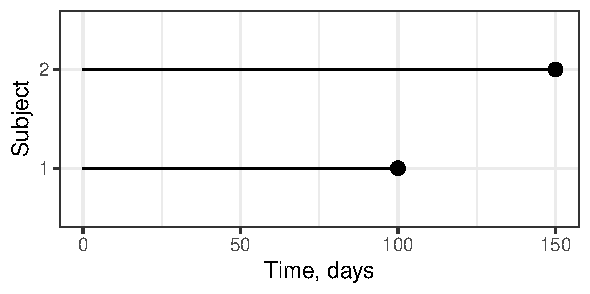
\includegraphics[width=0.6\textwidth]{../curve-cox/timeplot_1_light.pdf}
	\caption{
		An example of time-to-event data. Two subjects are followed from time 0. Subject 1 experiences the even at time 100. Subject 2 experiences the event at time 150.
	}
	\label{CoxExampleFull}
\end{figure}

Since subject 2 got infected later (i.e., ``survived'' for longer), the covariate pattern (e.g., antibody titre) of subject 2 would be considered by the model to be more ``protective'' than that of subject 1. That is, their covariates would be consistent with a reduced hazard. Since we assume that at most one infection is possible for any subject, both subjects are no longer at risk after the event. For subject 1, $t=100,\ Y=1$. For subject 2, $t=150,\ Y=1$. For any subject who does not get infected, $t$ would be their total follow-up time and $Y=0$.

If subjects are not at risk for all of their follow-up time (e.g., not exposed to the virus), then the total follow-up time may be misleading as illustrated in Figure \ref{CoxExamplePartial}. Taking the actual time at risk into account would lead to the opposite conclusion in this example --- it is subject 1 who is more ``protected'' since they were at risk for longer.

\begin{figure}[htp]
	\centering
	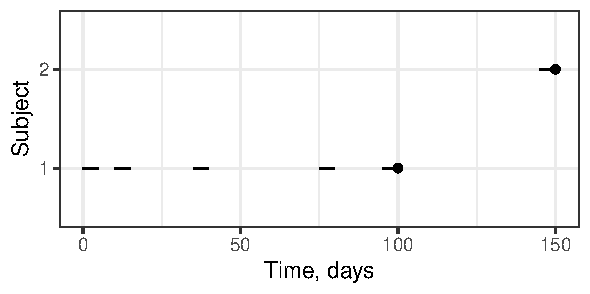
\includegraphics[width=0.6\textwidth]{../curve-cox/timeplot_2_light.pdf}
	\caption{
		An example of time-to-event data. Two subjects are followed from time 0. Subject 1 experiences the even at time 100. Subject 2 experiences the event at time 150. Subject 1 was at risk of the event for a total of 5 days. Subject 2 was at risk of the event for a total of 25 days.
	}
	\label{CoxExamplePartial}
\end{figure}

If follow-up time is completely unrepresentative of true time at risk, the Cox model will not produce meaningful results. However, if the total time of follow-up is assumed to be, on average, proportional to the total time at risk (e.g., subjects who are followed up for longer can be expected to have been exposed for longer) then the situation illustrated in Figure  \ref{CoxExamplePartial} will be ``averaged out'' and the model may still produce meaningful results.

To investigate the behaviour of the estimates when time of follow-up is not the same as time at risk but is proportional to it, we generated a simulated dataset, based on the following model:

\begin{align*}
	\begin{gathered}
		T \sim \text{Exponential}(\text{rate} = \lambda) \\
		h(t) = \lambda \\
		\text{log}\lambda = -3 - 1.5 X \\
		X \sim N(2, 2^2)
	\end{gathered}
\end{align*}

Where $T$ is the survival time, $h$ is the hazard function and $X$ is the true log-titre measurement.

Maximum time of follow-up was set to 100 days. Each individual was assigned a proportion of the follow-up time they were exposed to the virus (time-at-risk proportion). This proportion was generated from $\text{Beta}(\mu \kappa, (1 - \mu) \kappa)$ where $\mu$ is the expected proportion for the population and $\kappa$ is inversely proportional to the variance of the time-at-risk proportion. Smaller $\kappa$ values result in larger heterogeneity of exposure in the population. An individual's true time-at-risk was 100 (maximum follow-up) times their time-at-risk proportion. When $\mu = 1$, the time-at-risk proportion was always 1 (regardless of $\kappa$) to represent the ideal context of follow-up time being equal to time-at-risk.

A random number generated for each individual by $\text{Exponential}(\text{rate} = \text{exp}(-3 - 1.5 X_{\text{logtitre}}) )$ represented the time it would take that individual to experience the event (get infected), that is "survival" time. If survival time was greater than time-at-risk, the individual was "not infected" and their follow-up time was 100 (i.e., this was a right-censored observation). If survival time was smaller than time-at-risk, the individual was "infected" and their follow-up time was their survival time divided by their time-at-risk proportion.

For example, take a subject whose true survival time is 15, and time-at-risk proportion is 0.25. This individual can be at risk for at most 25 days over the 100-day follow-up period. Since their survival time is less than 25, this individual gets infected. Since their time-at-risk proportion is 0.25, we assume that they would have been exposed for 15 days (required for infection) in 60 days of follow-up (because 60 * 0.25 = 15). Thus for this individual $Y=1, t=60$.

Each simulation included 10,000 observations and was run 10,000 times at each of the following values of $\mu$: 0.01, 0.1, 0.2, 0.3, 0.4, 0.5, 0.6, 0.7, 0.9, 1 and at each of the following values of $\kappa$: 0.5, 1, 10, 100, 1000. The Cox proportional hazards model was fit to each simulated dataset. From 10,000 simulations at each combination of values of $\mu$ and $\kappa$, the mean of the estimated coefficient and its standard deviation were saved. The results are summarised in Figure \ref{CoxSimResults}.

In the ideal case ($\mu = 1$) the estimate is unbiased and has the smallest error. As the proportion of time at risk decreases, bias is introduced. More bias is introduced when $\kappa$ is small, i.e. when there is a larger amount of heterogeneity of exposure. When exposure is very similar for all members of the population (large $\kappa$), the model estimate has minimal bias across the range of $\mu$.

\begin{figure}[htp]
	\centering
	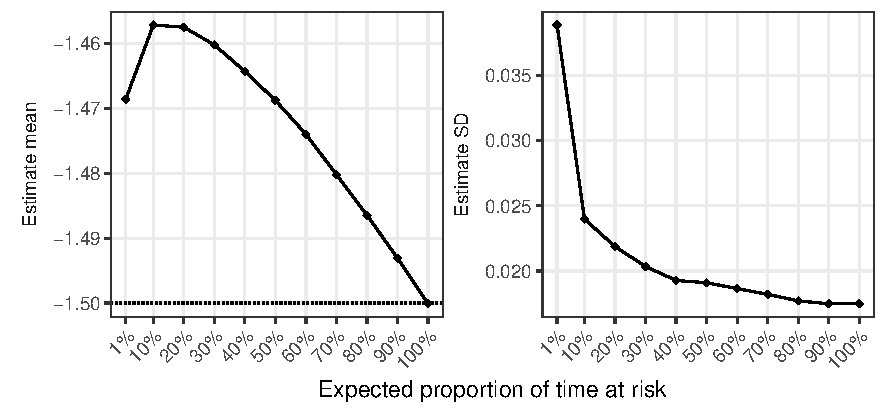
\includegraphics[width=1\textwidth]{../cox-tarprop/plot/risk.pdf}
	\caption{
		The results of fitting a Cox PH model to the time-to-event simulations. For each combination of $\mu$ and $\kappa$, the relative bias of the mean of the estimate (top panel) is shown as well the standard deviation of the estimate (bottom panel) obtained from 10,000 simulations. Lines are coloured according to the value of $\kappa$. Points represent the values for which the simulations were performed.
	}
	\label{CoxSimResults}
\end{figure}

The results in Figure \ref{CoxSimResults} show that the Cox PH model can produce (almost) unbiased estimates when time-at-risk is not the same as time-of-follow-up when two assumptions are satisfied. First is that time-at-risk is proportional to time-of-follow-up. Second is that exposure in the population is not overly heterogeneous, e.g. if subjects are expected to have been exposed for 20\% of their follow-up time then each individual subject was exposed for close to 20\% of their follow-up time (corresponds to simulations at $\kappa = 1000,\ \kappa = 100$) rather than having 20\% of the subjects almost always exposed and 80\% almost never exposed (corresponds to simulations at $\kappa = 0.5,\ \kappa = 1$).

The assumption of time at risk being proportional to time of follow-up is likely to hold when everyone in the sample is followed through a period of similar disease activity. There may still be subjects who are not exposed (or over-exposed), but as long as the level of exposure does not correlate with the covariates of interest (e.g., antibody titres), then with a large enough sample size the average exposure for any covariate pattern (e.g., antibody titre level) should be proportional in the same way to the time of follow-up. If the disease is seasonal, the start of follow-up can be set to the start of the season. For those who do not get infected, end of follow-up can then be the end of the season. For those who do get infected, end of follow-up can be the infection time assuming that infection grants immunity for the rest of the season. An illustration is in Figure \ref{CoxIdeal}.

\begin{figure}[htp]
	\centering
	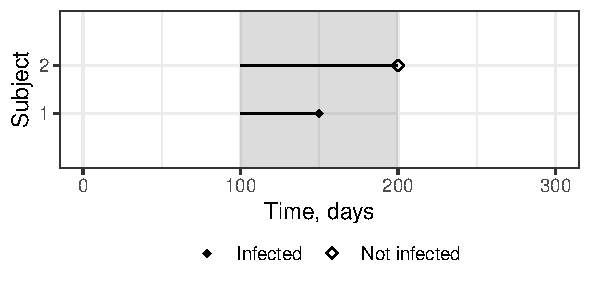
\includegraphics[width=0.59\textwidth]{../curve-cox/timeplot_3_light.pdf}
	\caption{
		An illustration of a pattern of follow-up where the assumption of true time at risk being proportional to time of follow-up is likely to hold. The shaded region marks the period of time when the disease is active. Both subject's follow-up starts at the beginning of the disease season (activity). Subject 1 gets infected at 150 days, their follow-up would end there assuming infection grants immunity (their total recorded time of follow-up would be 50 days). Subject 2 does not get infected through the season, their time of follow-up ends at the end of the season (their total recorded time of follow-up would be 100 days).
	}
	\label{CoxIdeal}
\end{figure}

This assumption will likely not hold if, with a seasonal disease, there are people in the sample whose follow-up starts before the season as shown in Figure \ref{CoxNotIdeal}. For those with earlier follow-up start, their follow-up time will be large regardless of their titres (since they spend a proportion of that time not being at risk). This should make it seem like the titres have a smaller effect than they actually do thus biasing the estimate of titre effect towards the null.

\begin{figure}[htp]
	\centering
	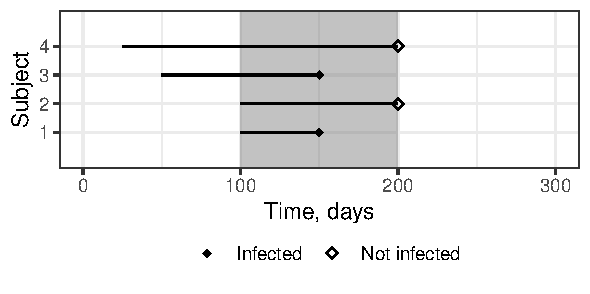
\includegraphics[width=0.59\textwidth]{../curve-cox/timeplot_4_light.pdf}
	\caption{
		An illustration of a pattern of follow-up where the assumption of true time at risk being proportional to time of follow-up is likely to not hold. The shaded region marks the period of time when the disease is active. Subject 1 gets infected at 150 days, at which point their follow-up would end if it can be assumed that infection grants immunity (their total recorded time of follow-up would be 50 days). Subject 2 does not get infected within the season, their follow-up ends at the end of the season (their total recorded time of follow-up would be 100 days). For subjects 3 (recorded follow up of 100 days) and 4 (recorded follow-up of 175 days) follow-up commenced prior to season onset.
	}
	\label{CoxNotIdeal}
\end{figure}

To demonstrate this problem, we performed a simulation study using the same procedure as described above, except a proportion of the subjects were randomly chosen to have their follow-up started earlier. For those randomly chosen, a uniform random number between 0 and 200 (days) was added to their recorded follow-up time. Time-at-risk proportion was always 1. This means that the subjects' follow-up time was equal to their time-at-risk unless they were chosen to have their follow-up started earlier and hence artificially extended.

The bias resulting from varying the proportion of the sample with earlier follow-up is shown in Figure \ref{CoxSimLong}. The estimate is unbiased when follow-up starts at the start of the season for all subjects. Bias towards the null increases rapidly even when only a small (10\%) proportion of the sample has started follow-up prior to the season. For this reason, it would be advisable to record follow-up time in such a way that true unobservable time at risk can be reasonably expected to be proportional to the recorded time of follow-up (i.e., the longer a subject is followed, the longer they are likely to have been at risk).

\begin{figure}[htp]
	\centering
	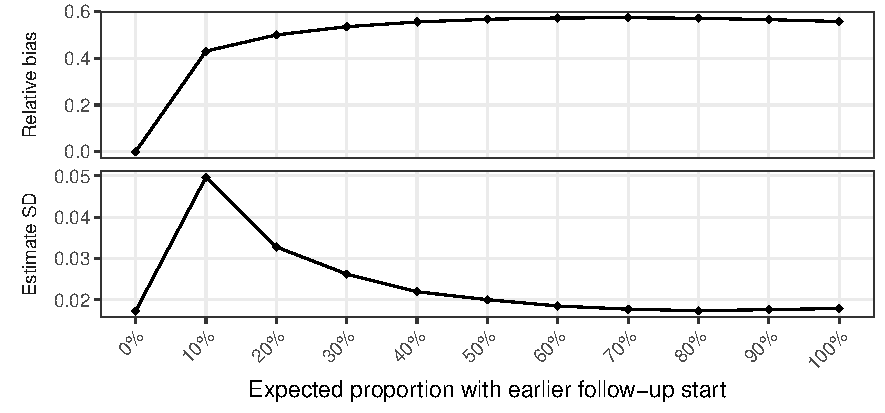
\includegraphics[width=1\textwidth]{../cox-tarprop/plot/long.pdf}
	\caption{
		The results of time-to-event simulations. For each proportion of the sample with earlier follow-up start, the mean of the estimated coefficient (top panel) is shown as well as the standard deviation of that coefficient (bottom panel) from 10,000 simulations. Points represent the values of expected proportion for which the simulations were performed.
	}
	\label{CoxSimLong}
\end{figure}


%------------------------------------------------------------------------------
\subsection{Logistic regression}

A potentially large problem with the application of the logistic model to antibody data is that low antibody titres do not necessarily correlate with a high probability of infection (which is one of the model's assumptions). This assumption of baseline risk of 1 can be justified if it is the case that subjects with low antibody titres always (or almost always) get infected. If a large proportion of subjects with low titres do not get infected, this assumption is not justified and this model will produce a poor fit.

If the baseline risk cannot justifiably be assumed to be 1, the fitted probability curve will be flatter than the true curve, thereby misrepresenting the true probability of infection across the titre range as depicted in Figure \ref{LogisticFit}. Thus, ignoring the baseline risk assumption will lead to poor model fit and hence biased estimates of titre effect.

\begin{figure}[htp]
	\centering
	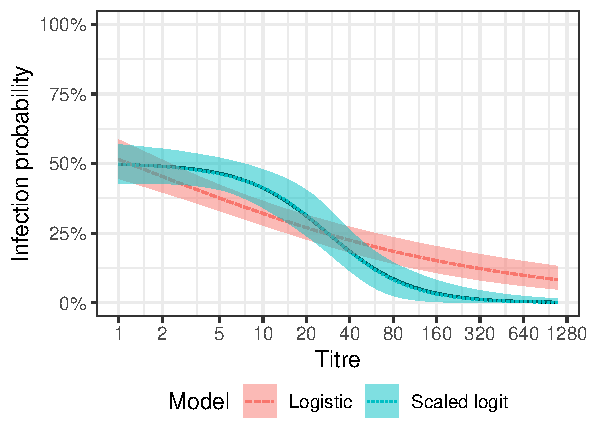
\includegraphics[width=0.6\textwidth]{../logistic-plot/predsplot.pdf}
	\caption{
		An illustration of a bad fit of the logistic model. The solid line ($0.5\ \text{logit}^{-1}(5 - 1.5 X)$) is the true probability curve where the baseline risk is 0.5. The dashed line is the expected fitted probability curve from standard logistic regression. The dotted line is the fitted probability curve from scaled logistic regression. The shaded regions are the 95\% confidence intervals. The expected curves and CIs was obtained from 10,000 simulations each with 500 observations simulated from the true curve. The models were fitted to each simulated dataset and the means of the regression estimates were taken from all simulations.
	}
	\label{LogisticFit}
\end{figure}

Estimating the baseline risk in the above model leads to the scaled logit model.


%------------------------------------------------------------------------------
\subsection{Scaled logistic regression}

The model still assumes that low probability bound is 0 (i.e. that high titres correlate with immunity in a univariate model). This assumption is justified if there is a reasonable number of people in the sample who have high titres and none (or very few) of whom get infected. In the Ha Nam data (Figure \ref{fig:hanam-hi-summ-h3n2}), no subject with a titre above 160 got infected in the corresponding season. For the Ha Nam data, the assumption of immunity at high titres is not unreasonable.

Compared to logistic regression, the scaled logit model requires a larger sample size. This is because the scaled logit model estimates an additional parameter. Hence for the same sample size, estimates from the scaled logit model will have larger standard errors.

Figures \ref{SclrSE}, \ref{SclrConv} and \ref{SclrMean} summarise 10,000 simulation results from the model

\begin{align*}
	\begin{gathered}
		\frac{0.5}{1 + \text{exp}(-5 + 1.5 X)} \\
		X \sim N(2, 2^2)
	\end{gathered}
\end{align*}

Figure \ref{SclrSE} shows that standard errors of the regression estimates were consistently higher with the scaled logit model.

Figure \ref{SclrConv} shows that in order to reliably converge (under the chosen true parameter values) the scaled logit model required the sample size to be over 500. The standard logistic model always converged.

The bias of the scaled logit estimates evident in Figure \ref{SclrMean} is likely due to the fact that the subset of the simulated datasets for which the scaled logit model converged is not a random subset. Datasets for which the scaled logit model is more likely to converge have certain properties, e.g. a large number of infections, a large number of subjects with detectable titres. Label these as "informative" datasets. Informative datasets are balanced out by simulated datasets where the opposite properties occur --- small infection numbers, small numbers with detectable titres. Label these "non-informative" datasets. With a large enough sample size, we can obtain estimates from both the informative and the non-informative datasets. With a small sample size, we can obtain estimates only from the informative datasets (the model does not converge for the non-informative), i.e. a non-random subset of simulated data. Aggregating estimates only over the informative datasets leads to bias.

\begin{figure}[htp]
	\centering
	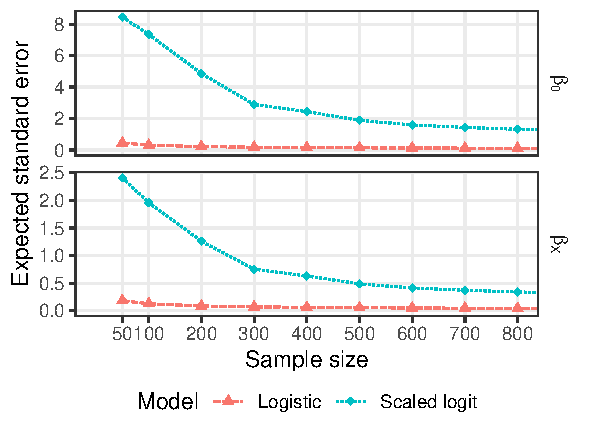
\includegraphics[width=0.69\textwidth]{../logistic-plot/vary_nsam_se.pdf}
	\caption{
		Simulation results of fitting the standard logistic and the scaled logit models to the same simulated datasets. 10,000 datasets were simulated. Shown is the mean standard error of the regression estimates from the standard logistic (the dashed line) and the scaled logit (the dotted line). Points indicate parameter values at which the simulations were performed.
	}
	\label{SclrSE}
\end{figure}

\begin{figure}[htp]
	\centering
	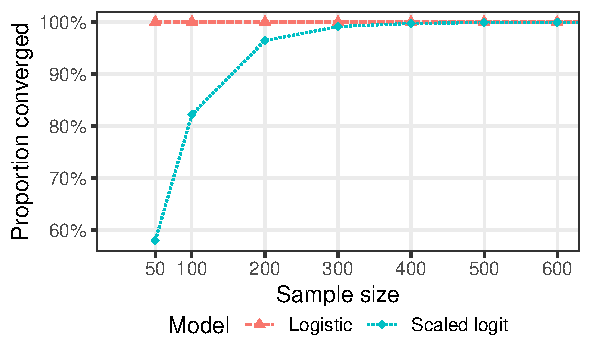
\includegraphics[width=0.69\textwidth]{../logistic-plot/vary_nsam.pdf}
	\caption{
		Simulation results of fitting the standard logistic and the scaled logit models to the same simulated datasets. 10,000 datasets were simulated. Shown is the proportion of successful attempts to fit the standard logistic (the dashed line) and the scaled logit (the dotted line) model. Points indicate parameter values at which the simulations were performed.
	}
	\label{SclrConv}
\end{figure}

\begin{figure}[htp]
	\centering
	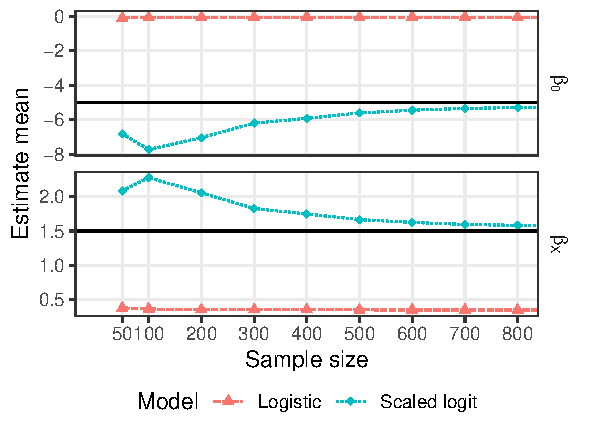
\includegraphics[width=0.69\textwidth]{../logistic-plot/vary_nsam_mean.pdf}
	\caption{
		Simulation results of fitting the standard logistic and the scaled logit models to the same simulated datasets. 10,000 datasets were simulated. Shown is the mean of the regression estimates from the standard logistic (the dashed line) and the scaled logit (the dotted line). Points indicate parameter values at which the simulations were performed. The solid lines are the true parameter values.
	}
	\label{SclrMean}
\end{figure}

When the unexposed subset of the population is present in the sample, the baseline risk $\lambda$ decreases. This does not necessarily bias the estimates of $\beta_0$ and $\beta_X$ but it can increase their standard errors.

To demonstrate the effect of including the unexposed population into the analysis on the standard errors of the parameter estimates, we simulated 10,000 observations from the model

\[
	\begin{gathered}
		P(Y=1) = \frac{P(E=1)\text{exp}(\theta)}{(1+\text{exp}(\theta))(1+\text{exp}(\beta_0+\beta_X X))} \\
		\theta = \text{log}(\frac{\lambda}{1-\lambda}) \\
		\lambda = 0.5 \quad \beta_0 = -5 \quad \beta_T = 1.5 \\
		X \sim N(2, 2^2)
	\end{gathered}
\]

at the following values of \(P(E=1)\): 0.1, 0.2, 0.3, 0.4, 0.5, 0.6, 0.7, 0.8, 0.9, 1.

We then fit the scaled logit model using maximum likelihood to all data (general population, unexposed included) and the subset with just the exposed (unexposed excluded). The results of 10,000 simulations at each value of \(P(E=1)\) are in Figure \ref{fig:sclr-lowbase}.

\begin{figure}[htp]
	\centering
	\includegraphics[width=1\textwidth]{../sclr-lowbase/sim-plot/plot2.pdf}
	\caption{
		The results of 10,000 simulations at each parameter combination. Points represent values at which simulations were performed. Points and lines are coloured based on the estimated term they belong to. The solid lines and triangles show estimated mean (left panel) and mean standard error (right panel) of estimates obtained from fitting models to the exposed population (i.e.,~unexposed excluded). The dashed lines and rhombi show the same for the general population (i.e.,~unexposed included).
	}
	\label{fig:sclr-lowbase}
\end{figure}

As expected, including the unexposed into the analysis has the effect of lowering the estimated baseline probability but has no appreciable effect on the expected estimates of the other parameters.

Including the unexposed into the analysis also has the effect of increasing the expected standard errors of the \(\beta_0\) and $\beta_X$ parameters (especially the intercept \(\beta_0\)) by 5-10\% when the exposed proportion is less then 50\%. As a result, it is advisable to limit the sample to those exposed, if possible.


%==============================================================================
\section{Application to real data}

We will use Ha Nam study data from 2009 to 2015 consisting of the subjects' pre-season HI titre measurements against the H3N2 virus as well as the subjects' H3N2 infection status in the season following the titre measurement. The lowest detectable HI titre was 10 (lowest dilution used), the highest --- 1280 (highest dilution used), and measurements within the detectable range were censored to intervals $[10, 20), [20, 40), ..., [640, 1280)$. Infection status was defined as either PCR-confirmed infection or a 4-fold HI titre rise comparing after-season titres to before-season titres. This Ha Nam data subset is depicted in Figure \ref{fig:hanam-hi-summ-h3n2}.

We will use Kiddivax study data consisting of the titre measurements taken against the B Victoria virus and the subjects' B Victoria infection status following the measurements. The lowest detectable HI titre was 10 (lowest dilution used) and HI measurements above 10 were censored to intervals $[10, 20), [20, 40), ..., [2560, 5120)$. No subject had a titre above 2560 against the B Victoria virus. Infection status was defined as PCR-confirmed infection. This Kiddivax data subset is depicted in Figure \ref{fig:kiddivax-main-summ}.

\begin{figure}[htp]
    \centering
    \includegraphics[width=1\textwidth]{../data-plot/hanam-hi-summ-h3n2.pdf}
    \caption{
        Ha Nam cohort data for the H3N2 virus from 2009 to 2015. Numbers next to points are the total number of observations in the corresponding group. The left panel shows data for the entire cohort. The right panel shows data from households with at least one infection in a given season. The measurement of 5 corresponds to titres below detectable levels.
    }
    \label{fig:hanam-hi-summ-h3n2}
\end{figure}

\begin{figure}[htp]
    \centering
    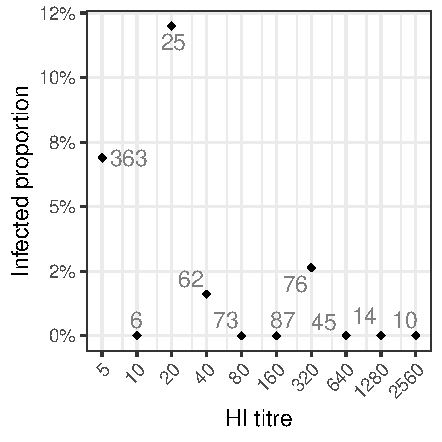
\includegraphics[width=0.5\textwidth]{../data-plot/kiddyvax-main-summ.pdf}
    \caption{
        Kiddivax study data for the B Victoria virus. Numbers next to points are the total number of observations in the corresponding group. The measurement of 5 corresponds to titres below detectable levels.
    }
    \label{fig:kiddivax-main-summ}
\end{figure}


%------------------------------------------------------------------------------
\subsection{Cox proportional hazards}

The Cox PH model was applied to the Kiddivax data. Subjects were tracked from the start of follow-up to either infection (if they were infected) or end of follow-up (if they were not infected). This analysis assumed that all subjects were followed through a period of similar disease activity and were similarly exposed. The resulting protection curve (relative to the titre of 5) is in Figure \ref{fig:kiddyvaxmain-cox}.

\begin{figure}[htp]
    \centering
    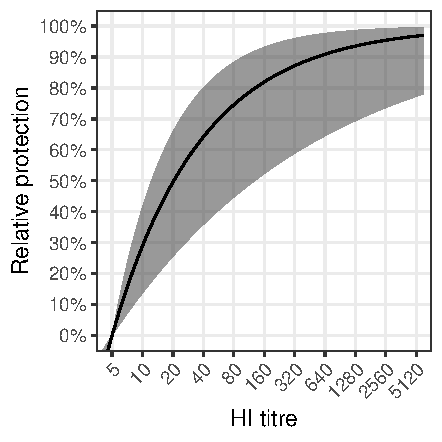
\includegraphics[width=0.5\textwidth]{../fit-cox-plot/kiddyvaxmain-bvic.pdf}
    \caption{
        Fitted relative-to-5 protection curve and confidence interval from the Cox proportional hazards model fit to B Victoria subset of Kiddivax data (shown in Figure \ref{fig:kiddivax-main-summ}). The solid line is the point estimates. The shaded region is the 95\% confidence interval.
    }
    \label{fig:kiddyvaxmain-cox}
\end{figure}


%------------------------------------------------------------------------------
\subsection{Logistic regression}

The logistic model was applied to both the Kiddivax and the Ha Nam data.

The resulting protection curve for Kiddivax is in Figure \ref{fig:kiddyvaxmain-prot-lr} and for Ha Nam --- in Figure \ref{fig:hanam-prot-lr}. The resulting relative-to-5 protection curve for Kiddivax is in Figure \ref{fig:kiddyvaxmain-prot-rel-lr-boot} and for Ha Nam --- in Figure \ref{fig:hanam-prot-rel-lr-boot}.

\begin{figure}[htp]
    \centering
    \includegraphics[width=0.5\textwidth]{../preds-plot/kiddyvaxmain-lr-bvic.pdf}
    \caption{
        Fitted protection curves and confidence intervals from the standard logistic model fit to Kiddivax data. The solid line is the point estimates. The shaded region is the 95\% confidence interval.
    }
    \label{fig:kiddyvaxmain-prot-lr}
\end{figure}

\begin{figure}[htp]
    \centering
    \includegraphics[width=0.5\textwidth]{../preds-plot/kiddyvaxmain-lr-boot-rel-bvic.pdf}
    \caption{
        Fitted relative-to-5 protection curves and confidence intervals from the standard logistic model fit to the B Victoria subset of Kiddivax data. The solid line is the point estimates. The shaded region is the 95\% confidence interval. The bounds for the confidence interval were obtained by using the bootstrap method (10,000 samples).
    }
    \label{fig:kiddyvaxmain-prot-rel-lr-boot}
\end{figure}

\begin{figure}[htp]
    \centering
    \includegraphics[width=0.8\textwidth]{../preds-plot/hanam-hi-lr-h3.pdf}
    \caption{
        Fitted protection curves and confidence intervals from the standard logistic model fit to Ha Nam data. The solid line is the point estimates. The shaded region is the 95\% confidence interval.
    }
    \label{fig:hanam-prot-lr}
\end{figure}

\begin{figure}[htp]
    \centering
    \includegraphics[width=0.8\textwidth]{../preds-plot/hanam-hi-lr-boot-rel-h3.pdf}
    \caption{
        Fitted relative-to-5 protection curves and confidence intervals from the standard logistic model fit to the H3N2 subset of the Ha Nam data. The solid lines are the point estimate. The shaded region is the 95\% confidence interval. The bounds for the confidence interval were obtained by using the bootstrap method (10,000 samples).
    }
    \label{fig:hanam-prot-rel-lr-boot}
\end{figure}

While the relative-to-5 protection curves appear more plausible than the relative-to-baseline protection curves, both result from fitting a model with an unsatisfied assumption (baseline of 1) and neither method of generating protection curves from logistic regression model reliably produces accurate results. In addition, the high confidence in the results is misplaced as it is a result of a string assumption on the data that is unfounded.

The relative-to-5 curves present an additional problem. The curve shows how much ``better'' different titres are at protecting against infection than the titre of 5.
There is nothing inherently special about this threshold of 5. Its choice is based on the lower dilution of 10 which is necessitated by the pre-treatment of sera. The curves may look substantially different if a different threshold (e.g. 10 or 1) is chosen. This hampers the interpretability and comparison of results.


%------------------------------------------------------------------------------
\subsection{Scaled logistic regression}

The scaled logit model was applied to both the Kiddivax and the Ha Nam data.

The resulting protection curve for Kiddivax is in Figure \ref{fig:kiddyvaxmain-prot-sclr} and for Ha Nam --- in Figure \ref{fig:hanam-prot-sclr}.

\begin{figure}[htp]
    \centering
    \includegraphics[width=0.5\textwidth]{../preds-plot/kiddyvaxmain-sclr-bvic.pdf}
    \caption{
        Fitted protection curves and confidence intervals from the scaled logit model fit to Kiddivax data. The solid line is the point estimates. The shaded region is the 95\% confidence interval.
    }
    \label{fig:kiddyvaxmain-prot-sclr}
\end{figure}

\begin{figure}[htp]
    \centering
    \includegraphics[width=0.8\textwidth]{../preds-plot/hanam-hi-sclr-h3.pdf}
    \caption{
        Fitted protection curves and confidence intervals from the scaled logit model fit to Ha Nam data. The solid line is the point estimates. The shaded region is the 95\% confidence interval.
    }
    \label{fig:hanam-prot-sclr}
\end{figure}

Out of the three models, the scaled logit model appears to be most appropriate.
The Kiddivax data did not have enough information to produce useful estimates.


%==============================================================================
\section{Conclusion}

\begin{table}[htp]
\centering
\caption{Summary of the three considered models in terms of their application to antibody data}
\begin{tabular}{cp{25em}}
\toprule
Model & Potential problem \\
\midrule
Cox PH & Biased if follow-up time is not proportional to time at risk for everyone in the sample \\
Logistic & Biased if low antibody titres do not guarantee immunity \\
Scaled logit & Requires a large sample size. \\
\bottomrule
\end{tabular}
\end{table}

In this paper we have explored three different models for estimating protective antibody titres using data from influenza vaccine and infection studies.  We have shown that in the presence of good time-to-event data where every subject's follow-up time is at least proportional to their time at risk, the Cox model will likely perform best out the three models explored due to it having the least number of parameters allowing for more precise estimates. Absent such data, logistic regression may be appropriate if the assumption of everyone being infected at low antibody titres can be justified. If this assumption cannot be justified, which is probably the case for influenza studies, the scaled logit model can be applied but the sample needs to be fairly large (>500) in order to obtain useful estimates.


\pagebreak
%=============================================================================
\bibliography{bibliography}
All code is in github.com/khvorov45/model-comparison

\end{document}
